
\chapter{Traffic monitoring methods}

%%%%%%%%%%%%%%%%%%%%%%%%%%%%% Introduction %%%%%%%%%%%%%%%%%%%%%%%%%%%%%

\section{Introduction}

Traffic monitoring is a critical component of modern urban infrastructure, enabling efficient traffic management, accident prevention, and emergency response. With the rapid growth of urbanization and the increasing complexity of road networks, traditional traffic monitoring systems often struggle to provide real-time, scalable, and cost-effective solutions. In recent years, advancements in Unmanned Aerial Vehicle (UAV) technology and wireless communication systems have opened new possibilities for innovative traffic monitoring approaches. These methods leverage the flexibility, mobility, and adaptability of UAVs to address the limitations of ground-based systems, such as fixed cameras and sensors.

\vspace{\baselineskip} % Add a line space between paragraphs

This chapter explores six distinct methods for UAV-based traffic monitoring, each offering unique solutions to specific challenges in traffic surveillance. From real-time video relay systems to collaborative hotspot selection frameworks, these methods demonstrate the potential of UAVs to enhance traffic monitoring capabilities. The chapter begins with an overview of early systems like the Airborne Traffic Surveillance System (ATSS) and progresses to more advanced approaches, such as 5G-integrated UAV systems and cooperative traffic monitoring using multiple UAVs. Each method is analyzed in terms of its architecture, operational workflow, performance, and limitations, providing a comprehensive understanding of the current state of UAV-based traffic monitoring technologies.

\vspace{\baselineskip} % Add a line space between paragraphs

By examining these methods, this chapter highlights the transformative potential of UAVs in traffic management while also addressing the technical, regulatory, and environmental challenges that must be overcome for widespread adoption. The following sections delve into the details of each method, offering insights into their design, implementation, and real-world applicability.


%%%%%%%%%%%%%%%%%%%%%%%%%%%%% Method 1 %%%%%%%%%%%%%%%%%%%%%%%%%%%%%
\newpage

\section{Method 1: Airborne Traffic Surveillance System (ATSS)}
\label{sec:method1}

In \cite{srinivasan2004atss}, the University of Florida (UFL) research team, in collaboration with the Florida Department of Transportation (FDOT), developed the \textbf{Airborne Traffic Surveillance System (ATSS)}. This innovative system leverages \textbf{Unmanned Aerial Vehicles (UAVs)} and \textbf{microwave IP networks} to transmit highway surveillance data to a \textbf{Base Station (BS)}. The UAV captures video footage of traffic and transmits it in real-time. Two computers located in towers function as video encoders, while another computer at the State Emergency Operations Center receives and displays the strongest video signal. Figure \ref{fig:Methode_1_1} illustrates the system framework.

\begin{figure}[H]  
    \centering
    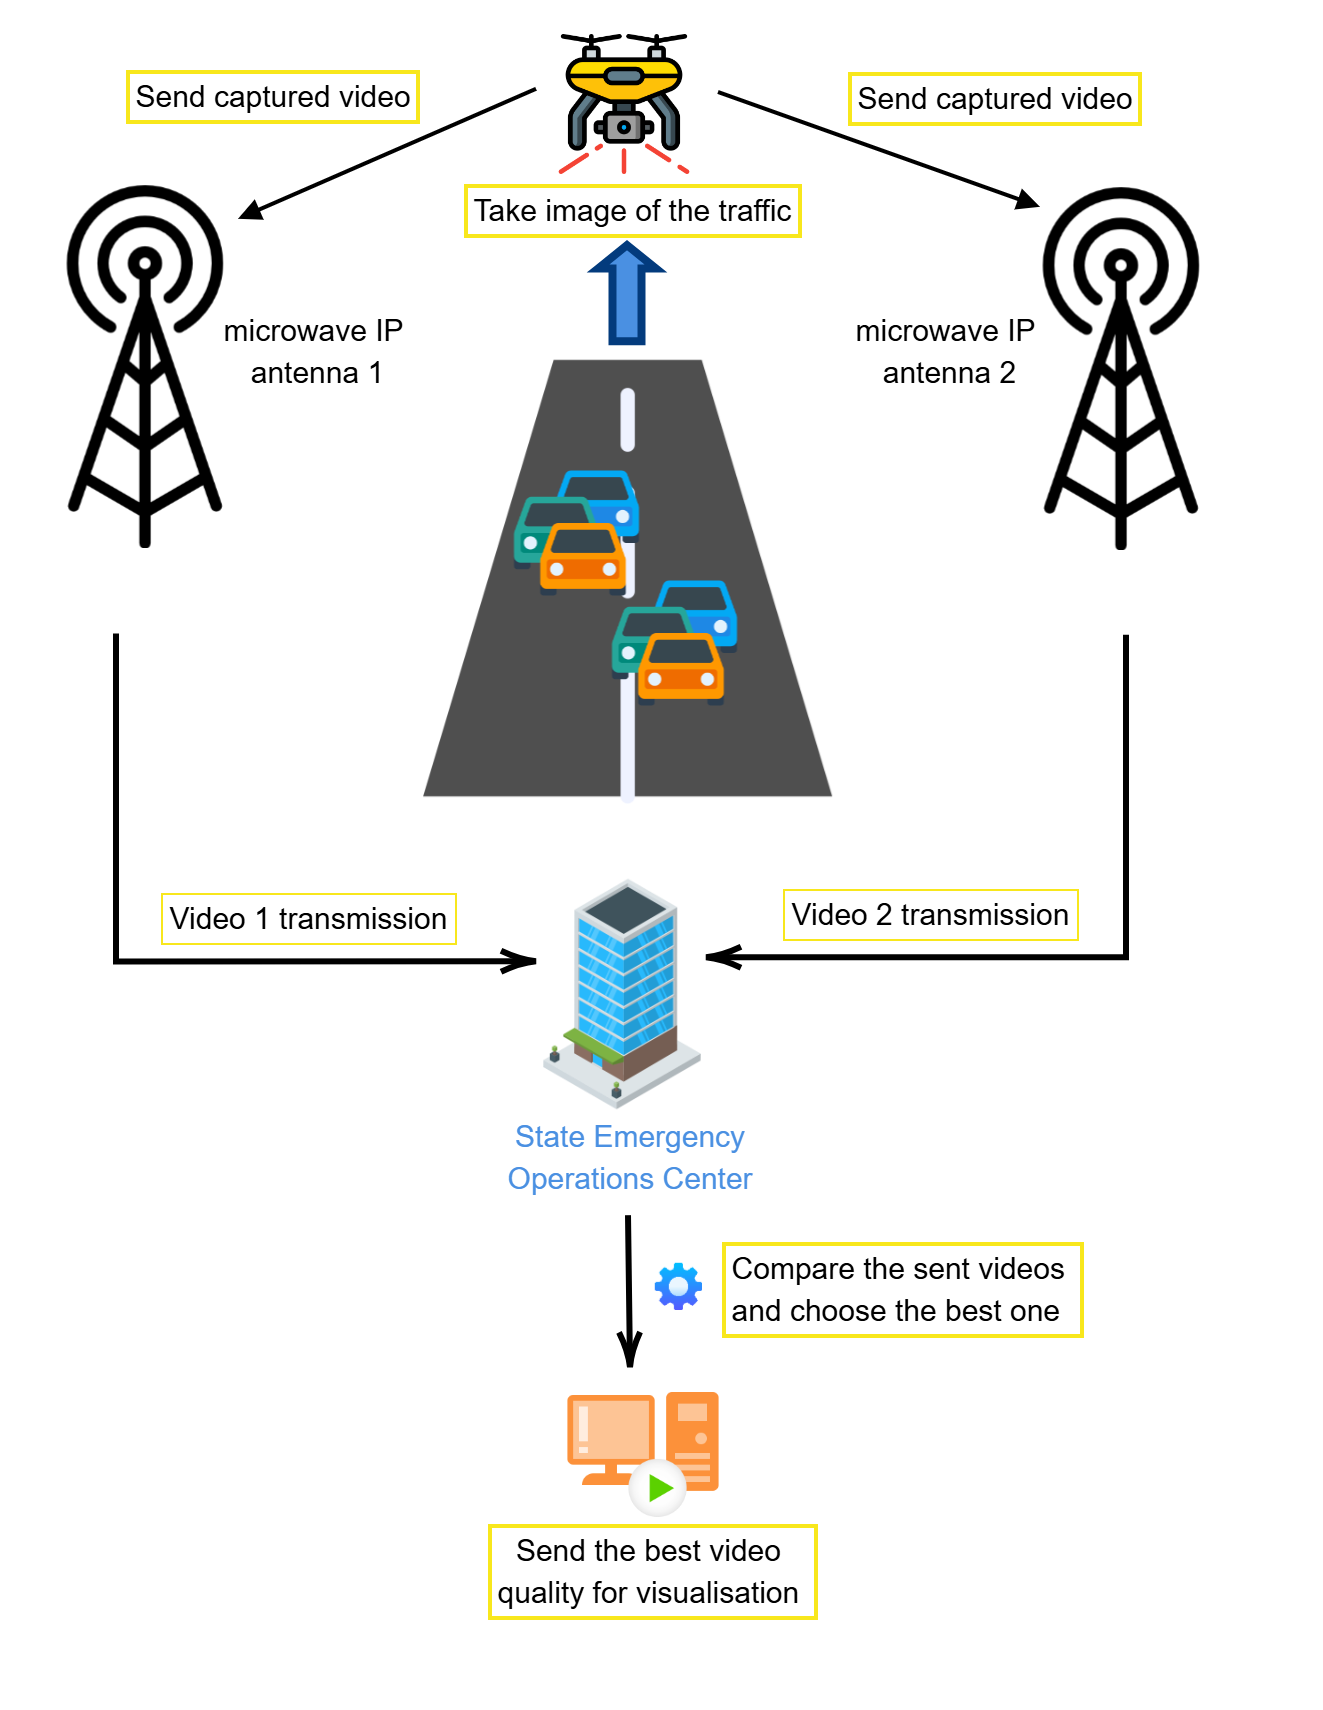
\includegraphics[width=0.7\textwidth]{Figures/Chapter3/Method1/1.png} % Adjust width as needed
    \caption{Airborne Traffic Surveillance System (ATSS) Architecture}
    \label{fig:Methode_1_1} % Reference label
\end{figure}

\subsection{Key Features of ATSS}
The ATSS represents a significant advancement in traffic monitoring, offering the following capabilities:
\begin{itemize}
    \item Real-time video capture and transmission of traffic conditions.
    \item Utilization of UAVs for flexible and scalable surveillance.
    \item Integration with microwave IP networks for data transmission.
    \item Centralized monitoring at the State Emergency Operations Center.
\end{itemize}

\subsection{Limitations of ATSS}
Despite its innovative approach, the ATSS faces several challenges that impact its effectiveness and scalability:
\begin{itemize}
    \item \textbf{Regulatory Constraints:} Federal Aviation Administration (FAA) restrictions limit UAV operations, requiring specific approvals and slowing deployment.
    \item \textbf{Communication Challenges:} Bandwidth limitations, signal reliability issues, and potential interference, especially in adverse weather conditions.
    \item \textbf{Energy and Flight Duration:} Limited battery life necessitates frequent landings and recharging, reducing operational efficiency.
    \item \textbf{Environmental Factors:} Strong winds, rain, and fog degrade video quality and affect UAV stability.
    \item \textbf{Real-Time Video Transmission:} Requires efficient data compression and robust network infrastructure to minimize delays and ensure reliability.
    \item \textbf{Operational Costs:} While more cost-effective than manned aircraft, UAV deployment involves expenses for equipment, trained personnel, and maintenance.
    \item \textbf{Privacy and Security Concerns:} Raises ethical and legal issues, necessitating strict regulations for data collection and surveillance.
\end{itemize}

\subsection{Future Potential}
Despite these limitations, UAV-based traffic monitoring holds significant promise. Future advancements, such as \textbf{AI-driven analysis}, \textbf{improved communication technologies (e.g., 5G)}, and \textbf{autonomous UAV operations}, could enhance its feasibility for large-scale implementation. These developments may address current challenges and unlock new possibilities for real-time traffic management.

\subsection{Conclusion}
The Airborne Traffic Surveillance System (ATSS) represents a pioneering approach to UAV-based traffic monitoring, offering real-time video capture and transmission through microwave IP networks. Despite its innovative design, the system faces challenges such as regulatory constraints, communication limitations, energy inefficiencies, and environmental sensitivities. However, future advancements in AI-driven analytics, 5G communication, and autonomous UAV operations hold the potential to address these limitations, making the ATSS a promising foundation for scalable and efficient traffic surveillance systems.

%%%%%%%%%%%%%%%%%%%%%%%%%%%%% Method 2 %%%%%%%%%%%%%%%%%%%%%%%%%%%%%

\section{Method 2: Video Relay Model Using Public Networks}
\label{sec:method2}

A comparable surveillance method was proposed in \cite{chen2007realtime}, where researchers developed a \textbf{video relay model} using existing public networks. This approach addresses the limitations of traditional traffic surveillance systems, such as the high cost and time-consuming installation of cameras on microwave towers along highways \cite{srinivasan2004atss}. Instead, this method leverages \textbf{mobile broadband connections} to transmit video footage directly to a ground base station (BS) located near the UAV. The efficiency of this method depends on the proximity of ground stations and the availability of a stable broadband network.

\vspace{\baselineskip} % Add a line space between paragraphs

\subsection{Ground Control Station and Network Setup}
A distinctive aspect of this project is the strategic placement of the ground control station near the highway, allowing seamless access to a roadside communication tower. This setup enables the use of the existing mobile broadband network to transmit surveillance video efficiently. The primary goal of video relaying is to send video signals from the UAV ground station in the field to control office computers. Since most of these computers are connected to the Internet, using the public Internet as the main network for video transmission simplifies the setup and reduces system requirements for end-user computers. Figure \ref{fig:method2_architecture} illustrates the proposed architecture.

\vspace{\baselineskip} % Add a line space between paragraphs

\begin{figure}[h]  % 'h' means place the figure "here" if possible
    \centering
    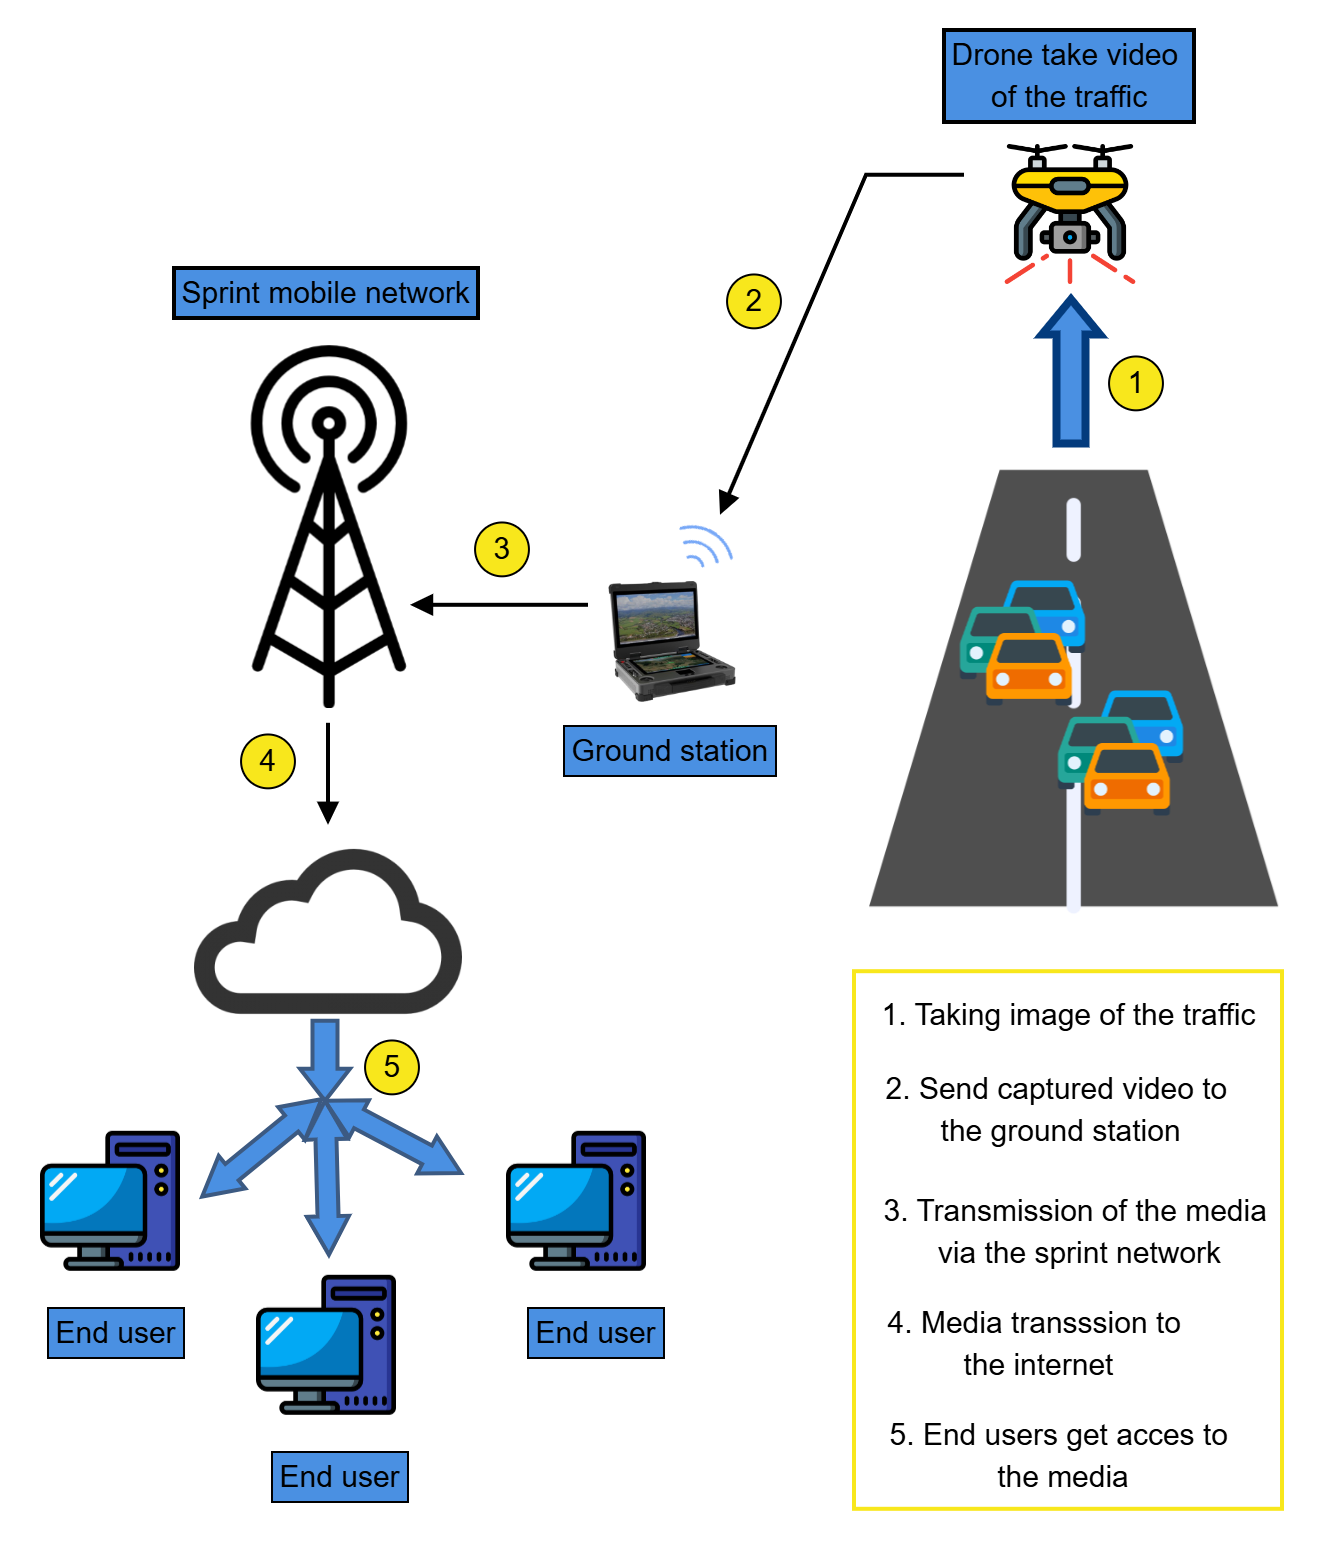
\includegraphics[width=0.7\textwidth]{Figures/Chapter3/Method2/1.png} % Adjust width as needed
    \caption{Proposed Architecture of the Video Relay Model}
    \label{fig:method2_architecture} % Reference label
\end{figure}

\vspace{\baselineskip} % Add a line space between paragraphs

\subsection{Operational Workflow}
The ground station, which consists of a laptop equipped with an antenna, is placed in the field to ensure that the UAV has a suitable flying range covering a section of the Interstate Highway. The best location for the ground station may not always have a wired Internet connection. However, since it is usually set up near the highway, it can take advantage of nearby cellular towers for communication. To send video over the Internet, the UAV ground station uses the nationwide \textbf{Sprint mobile broadband network}. The laptop at the ground station connects to this network using a wireless PC card, which acts as a bridge to the Internet. Once online, the transmitted video is received by the mobile base station through the Internet.

\vspace{\baselineskip} % Add a line space between paragraphs

One drawback of this approach is that the wireless connection in the Sprint mobile broadband network can slow down data transmission. In other words, the system's performance is limited by the available bandwidth in the wireless network. To address this limitation, researchers developed two methods for transmitting the video over the Internet.

\vspace{\baselineskip} % Add a line space between paragraphs

\subsection{Direct IP Address Sharing}
In the first method (see Figure \ref{fig:method2_architecture}), the UAV ground control laptop shares its IP address with end users, who can then use a media player to stream the video from that address. However, the Sprint mobile broadband service assigns a new IP address each time a connection is established. As a result, the IP address changes every time the ground control laptop reconnects to the Sprint network. This requires the ground crew to update and inform end users of the new IP address for each session, creating operational inefficiencies.

\vspace{\baselineskip} % Add a line space between paragraphs

\subsection{Server-Based Video Relay}
An improvement to the system involves using an additional server to manage the data connection. This server has a \textbf{fixed IP address}, which is known in advance by both the UAV ground control laptop and the end-user computers. The UAV ground control laptop streams the video to the server using this fixed IP address, and end users access the video from the same server. Besides real-time streaming, the server can also save the received video for later analysis. Additionally, it hosts the project website, which includes a page displaying the live video feed from the UAV camera. To handle both website hosting and incoming video streams, the server has multiple open network ports. However, using a server may introduce some delays in processing and could be affected by firewall restrictions.

\vspace{\baselineskip} % Add a line space between paragraphs

In this second method, the UAV ground control laptop transmits the video to the server through the mobile broadband network. The server then forwards the video to end-user computers using a wired Internet connection. The number of users who can watch the video at the same time depends on the server's wired connection speed, which is significantly higher than that of the wireless network. As a result, more users can access the video stream simultaneously with a stable data rate. This approach overcomes the limitations of the wireless connection, which is the main bottleneck for video transmission.

\vspace{\baselineskip} % Add a line space between paragraphs

\subsection{Limitations of the Method}
Despite its innovative approach, the video relay model using public networks has several limitations that need to be addressed for practical deployment:

\begin{itemize}
    \item \textbf{Bandwidth Constraints}: The system's performance is heavily dependent on the available bandwidth of the mobile broadband network. In areas with poor network coverage or high congestion, video transmission may suffer from delays or interruptions.
    
    \item \textbf{Operational Inefficiencies}: The direct IP address sharing method requires manual updates to inform end users of new IP addresses, leading to operational inefficiencies and potential delays in accessing video feeds.
    
    \item \textbf{Server Dependency}: The server-based relay method introduces additional complexity and cost. Delays in processing and potential firewall restrictions can impact the system's real-time performance.
    
    \item \textbf{Energy Consumption}: UAVs and ground stations rely on battery power, which limits their operational duration. Frequent recharging or battery replacement may be required, especially in large-scale deployments.
    
    \item \textbf{Environmental Factors}: Adverse weather conditions, such as heavy rain or strong winds, can affect UAV stability and the quality of video footage, reducing the system's reliability.
    
    \item \textbf{Scalability Issues}: While the system performs well in small-scale deployments, scaling it to cover larger areas or higher traffic volumes may introduce challenges in network organization and resource allocation.
\end{itemize}

\vspace{\baselineskip} % Add a line space between paragraphs

\subsection{Conclusion}
In conclusion, the video relay model using public networks represents a \textbf{cost-effective and scalable solution} for UAV-based traffic monitoring. While challenges such as bandwidth limitations and operational inefficiencies persist, the integration of server-based relay systems significantly enhances the method's feasibility and performance.


%%%%%%%%%%%%%%%%%%%%%%%%%%%%% Method 3 %%%%%%%%%%%%%%%%%%%%%%%%%%%%%


\section{Method 3: UAV-Based Traffic Surveillance with 5G Integration}
\label{sec:method3}

In \cite{khan2024smarttraffic}, researchers proposed a novel solution to address the weaknesses of SAHER, an automated traffic enforcement system used in Saudi Arabia. SAHER relies on cameras and radar technology to detect traffic violations such as speeding, running red lights, and lane violations. While effective, the system has several limitations:

\begin{itemize}
    \item Drivers often hide their license plates to avoid detection.
    \item Drivers warn others when they spot a speed camera.
    \item Drivers adhere to speed limits only in areas monitored by SAHER cameras.
    \item Drivers slow down near speed cameras but speed up afterward.
\end{itemize}

To overcome these challenges, the researchers proposed an \textbf{airborne traffic surveillance system} using drones (UAVs) and 5G technology. This system is structured into three layers, each serving a distinct purpose.

\vspace{\baselineskip} % Add a line space between paragraphs

\subsection{System Architecture}
The proposed system consists of three layers:

\begin{itemize}
    \item \textbf{Layer 1}: UAVs fly over highways, capturing video footage and GPS data, which are transmitted to a mobile police base station.
    \item \textbf{Layer 2}: 5G technology ensures a fast and stable connection between the UAVs and the police station.
    \item \textbf{Layer 3}: The system facilitates efficient highway traffic management.
\end{itemize}

\begin{figure}[H]  % 'h' means place the figure "here" if possible
    \centering
    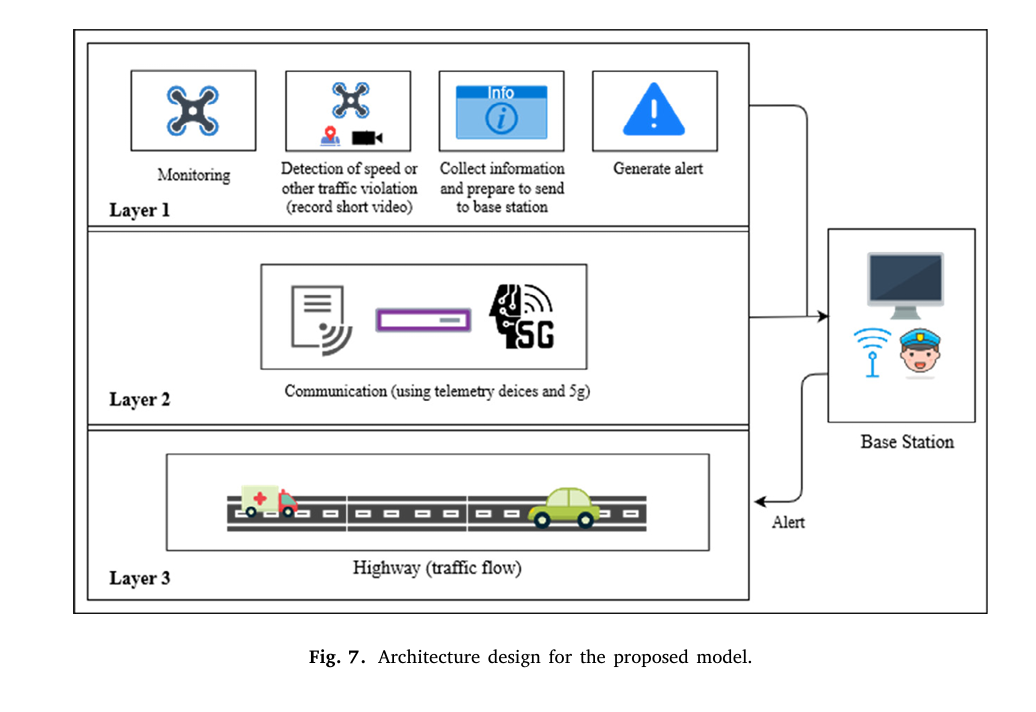
\includegraphics[width=0.7\textwidth]{Figures/Chapter3/Method3/1.png} % Adjust width as needed
    \caption{Proposed Architecture of the UAV-Based Traffic Surveillance System (Source: \cite{khan2024smarttraffic})}
    \label{fig:method3_architecture} % Reference label
\end{figure}

\vspace{\baselineskip} % Add a line space between paragraphs

\subsection{Traffic Monitoring and Violation Detection}
The UAV monitors highway traffic, detects violations, and ensures road safety. When a violation occurs, the system follows a two-step enforcement approach:

\begin{itemize}
    \item \textbf{First Violation}: The UAV issues a warning to the driver through an integrated communication system.
    \item \textbf{Repeated Violation}: If the driver commits the same offense again, the UAV records the details, issues a ticket using License Plate Recognition (LPR), and sends the information to the nearest base station for legal action.
\end{itemize}

\vspace{\baselineskip} % Add a line space between paragraphs

\subsection{Layer 1: UAV-Based Traffic Monitoring}
A UAV is deployed to monitor highways, equipped with an advanced camera and GPS tracking system. It continuously scans traffic for speeding and other infractions, recording real-time violations. When a violation is detected, the UAV captures a short video and logs the GPS coordinates. If it’s the driver’s first offense, the system issues a warning via an integrated module in the vehicle. The collected data is transmitted to the base station for further action. To counteract license plate tampering (e.g., covering plates with tape to evade detection), the base station maintains vehicle records and can take legal action when the vehicle reaches a designated checkpoint.

\vspace{\baselineskip} % Add a line space between paragraphs

\subsection{Layer 2: Communication Network}
This layer facilitates data transmission between the UAV and the base station using telemetry or modern communication technologies. With advancements in communication, \textbf{5G} is the preferred choice due to its high speed, broad coverage, and low latency. The system relies on 5G for seamless and real-time data exchange, ensuring efficient monitoring and response.

\vspace{\baselineskip} % Add a line space between paragraphs

\subsection{Layer 3: Highway Traffic Management}
This layer focuses on optimizing vehicle flow in the monitored areas. By integrating the UAV’s data with traffic control systems, authorities can make informed decisions to improve road safety and efficiency.

\vspace{\baselineskip} % Add a line space between paragraphs

\subsection{Algorithm for Traffic Monitoring}
The following algorithm, adapted from \cite{khan2024smarttraffic}, outlines the process of traffic monitoring and violation detection:




\begin{algorithm}[H]
    \caption{Traffic Monitoring and Rule Violation Detection (Source: \cite{khan2024smarttraffic})}
    \label{alg:traffic_monitoring}
    \textbf{Step 1:} Initialize\;
    
    \textbf{Step 2:} Start monitoring traffic\;
    
    \textbf{Step 3:} Detect speed and other traffic rule violations\;
    
    \textbf{Step 4:} \If{Rule violation found and first time}{
        \textbf{4.1} Generate warning and alert the driver\;
        \textbf{4.2} Record a short video and GPS coordinates\;
        \textbf{4.3} Send video and associated data to ground control station\;
    }
    
    \textbf{Step 5:} \ElseIf{Rule violation found}{
        \textbf{5.1} Record a short video and GPS coordinates\;
        \textbf{5.2} Send video and associated data to ground control station\;
        \textbf{5.3} Ground control station will process data and send to authorities\;
        \textbf{5.4} Go to Step 3\;
    }
    
    \textbf{Step 6:} \If{Flight time ended}{
        \textbf{6.1} Go to Step 8\;
    }
    \Else{
        \textbf{7.1} Go to Step 2\;
    }
    
    \textbf{Step 8:} Go to ground control station\;
    
    \textbf{Step 9:} Exit\;
\end{algorithm}

% \begin{algorithm}[H]
%     \caption{Traffic Monitoring and Rule Violation Detection (Source: \cite{khan2024smarttraffic})}
%     \label{alg:traffic_monitoring}
%     \textbf{Step 1:} Initialize\;
    
%     \textbf{Step 2:} Start monitoring traffic\;
    
%     \textbf{Step 3:} Detect speed and other traffic rule violations\;
    
%     \textbf{Step 4:} \If{Rule violation found and first time}{
%         \textbf{4.1} Generate warning and alert the driver\;
%         \textbf{4.2} Record a short video and GPS coordinates\;
%         \textbf{4.3} Send video and associated data to ground control station\;
%     }
    
%     \textbf{Step 5:} \ElseIf{Rule violation found}{
%         \textbf{5.1} Record a short video and GPS coordinates\;
%         \textbf{5.2} Send video and associated data to ground control station\;
%         \textbf{5.3} Ground control station will process data and send to authorities\;
%         \textbf{5.4} Go to Step 3\;
%     }
    
%     \textbf{Step 6:} \If{Flight time ended}{
%         \textbf{6.1} Go to Step 8\;
%     }
%     \Else{
%         \textbf{7.1} Go to Step 2\;
%     }
    
%     \textbf{Step 8:} Go to ground control station\;
    
%     \textbf{Step 9:} Exit\;
% \end{algorithm}

\vspace{\baselineskip} % Add a line space between paragraphs

\subsection{Limitations of the Proposed System}
Despite its innovative approach, the proposed UAV-based system faces several challenges:

\begin{itemize}
    \item \textbf{Higher Mobility}: The movement of UAVs can cause instability in the communication link, as the network must continuously adjust to their changing positions.
    \item \textbf{Line-of-Sight Interference}: UAVs rely on clear line-of-sight communication, and obstacles like buildings or terrain can block or degrade the signal.
    \item \textbf{Energy Constraints}: The limited battery life of UAVs restricts their ability to operate over long periods, especially in large or remote areas where frequent recharging or battery swaps are required.
\end{itemize}

These factors contribute to the complexity of cellular network planning and make the implementation of this system challenging.

\vspace{\baselineskip} % Add a line space between paragraphs

\subsection{Conclusion}
The proposed UAV-based traffic surveillance system with 5G integration represents a significant advancement in traffic monitoring and enforcement. While challenges such as mobility, line-of-sight interference, and energy constraints persist, the system's potential for real-time monitoring and efficient traffic management makes it a promising solution for future implementation.
    

%%%%%%%%%%%%%%%%%%%%%%%%%%%%% Method 4 %%%%%%%%%%%%%%%%%%%%%%%%%%%%%
 
    
\section{Method 4: Cooperative Traffic Monitoring Using Multiple UAVs}
\label{sec:method4}

In \cite{elloumi2018monitoring}, researchers introduced a cooperative traffic monitoring system using multiple UAVs. This system incorporates two distinct approaches: one focused on maximizing vehicle coverage and the other on detecting various traffic events, such as vehicle positions and speeds. While the first approach dynamically adjusts UAV trajectories based on the movement of targeted vehicle groups, the second relies on predefined vehicle mobility models to determine UAV paths. However, this multi-UAV system lacks real-time capabilities for identifying and reporting speed violations to the mobile police base station.

\vspace{\baselineskip} % Add a line space between paragraphs

\begin{comment}
    

\subsection{System Overview}
The objective of this solution is to track vehicles moving through urban roads, treating them as targets that require continuous monitoring. To design an effective UAV-based system, it is essential to:
\begin{itemize}
    \item Determine a suitable approach for gathering vehicle data.
    \item Strategically position UAVs across the designated area.
    \item Design optimized flight paths to maximize target coverage.
\end{itemize}

The primary challenge lies in determining the number of UAVs required to cover a city, assuming static UAV placement. Since deploying an unlimited number of UAVs is impractical, each UAV must cover multiple targets. One way to reduce the number of UAVs is by clustering targets and assigning one UAV to each cluster. This approach is similar to techniques used in sensor networks or Vehicular Ad-Hoc Networks (VANETs). Key parameters for clustering include target distances, velocities, and movement directions. A group is more stable if its members have similar velocities and move in the same direction.


\end{comment}



\vspace{\baselineskip} % Add a line space between paragraphs

\subsection{Key Components of the System}
The system is constracted through three main steps:

\subsubsection{Collecting Information About Vehicles}
Various parameters can be monitored and measured based on the devices deployed over the coverage area, including:
\begin{itemize}
    \item Vehicle position, speed, and direction.
    \item The number of vehicles in an area.
    \item The number of vehicles passing through specific points, such as intersections or crossings.
\end{itemize}

Specific events, such as speeding or traffic jams, are identified by changes in these parameters. For example:
\begin{itemize}
    \item Speeding is detected when a vehicle exceeds a set speed limit.
    \item Traffic jams are identified when the speed of multiple vehicles drops below a certain threshold.
\end{itemize}

In this research, \cite{elloumi2018monitoring} consider multiple UAVs equipped with image-processing capabilities that enable them to accurately measure these parameters. The UAVs are assumed to:
\begin{itemize}
    \item Always detect targets within their field of view, with no obstacles obstructing their line of sight.
    \item Temporarily adjust their altitude to avoid collisions.
    \item Exchange information about the vehicles they are tracking, including identifiers and positions.
\end{itemize}

\vspace{\baselineskip} % Add a line space between paragraphs

\subsubsection{Deploying UAVs Over Coverage Areas}
The key challenge is determining the number of UAVs required to effectively cover a city area. Since deploying an unlimited number of UAVs is impractical, each UAV must monitor multiple targets. To minimize the required number of UAVs, targets are grouped into clusters, with each UAV assigned to a specific cluster. The clustering process considers factors such as:
\begin{itemize}
    \item Distance between targets.
    \item Velocities of targets.
    \item Movement directions of targets.
\end{itemize}

An off-line algorithm (Algorithm 1) is proposed for this clustering, allowing system operators to estimate the UAV count. The algorithm inputs are shown in Table \ref{tab:clustering_inputs}. Three criteria are used for clustering:
\begin{itemize}
    \item Distance between the central target and potential group members (mandatory).
    \item Speed difference between targets (optional).
    \item Direction of movement (optional).
\end{itemize}

\begin{table}[H]
    \centering
    \begin{tabular}{|l|l|}
    \hline
    \textbf{Abbreviation} & \textbf{Description} \\ \hline
    Tnb & Targets numbers \\ \hline
    G & Groups members \\ \hline
    D & Max distance value \\ \hline
    V & Max speed difference \\ \hline
    Pt & Target position \\ \hline
    Mt & Target direction \\ \hline
    Vt & Target velocity \\ \hline
    compt & Covered targets \\ \hline
    Ttag & Target tag \\ \hline
    Tid & Target id \\ \hline
    Cid & Central target id \\ \hline
    Pc & Central target position \\ \hline
    Mc & Central target direction \\ \hline
    Ctag & Central target tag \\ \hline
    Vc & Central target speed \\ \hline
    \end{tabular}
    \caption{Input Parameters for Clustering Algorithm (Source: \cite{elloumi2018monitoring})}
\end{table}


\vspace{\baselineskip} % Add a line space between paragraphs

\begin{algorithm}[H]
    \caption{Clustering Algorithm}
    \label{alg:uniform_method}
    
    \textbf{Step 1:} Initialize $j \gets 1$, $\text{compt} \gets 0$\;
    
    \textbf{Step 2:} \While{$\text{compt} < T_{\text{nb}}$}{
        \textbf{2.1} \While{$C_{\text{tag}}(j) = 1$}{
            \textbf{2.1.1} Sample $P_c(j) \sim \text{Uniform}(P_t)$\;
            
            \textbf{2.1.2} Set $C_{\text{tag}}(j) \gets 1$\;
            
            \textbf{2.1.3} Set $G(j, j) \gets C_{\text{id}}(j)$\;
            
            \textbf{2.1.4} Increment $\text{compt} \gets \text{compt} + 1$\;
            
            \textbf{2.1.5} \For{$i = 1$ \KwTo $T_{\text{nb}}$}{
                \textbf{2.1.5.1} \If{$(T_{\text{tag}}(i) = 0) \land (i \neq j)$}{
                    \textbf{2.1.5.1.1} \If{$M_t(i) = M_c(j)$}{
                        \textbf{2.1.5.1.1.1} \If{$|V_t(i) - V_c(j)| < V$}{
                            \textbf{2.1.5.1.1.1.1} \If{$|P_t(i) - P_c(j)| < D$}{
                                \textbf{2.1.5.1.1.1.1.1} Set $G(j, i) \gets T_{\text{id}}(i)$\;
                                
                                \textbf{2.1.5.1.1.1.1.2} Increment $\text{compt} \gets \text{compt} + 1$\;
                                
                                \textbf{2.1.5.1.1.1.1.3} Set $T_{\text{tag}}(i) \gets 1$\;
                            }
                        }
                    }
                }
            }
            
            \textbf{2.1.6} Increment $j \gets j + 1$\;
        }
    }
    
    \textbf{Step 3:} End\;
\end{algorithm}

    

% \begin{algorithm}[H]
% \caption{Clustering Algorithm (Source: \cite{elloumi2018monitoring})}
% \label{alg:uniform_method}
% \begin{algorithmic}[1]
% \State $j = 1$; $\text{compt} = 0$;
% \While{$\text{compt} < T_{\text{nb}}$}
%     \While{$C_{\text{tag}}(j) == 1$}
%         \State $\bigcup\limits_{c(j)} P_c(j) = \text{Uniform } (P_t)$;
%         \State $C_{\text{tag}}(j) = 1$; $G(j, j) = C_{\text{id}}(j)$;
%         \State $\text{compt} = \text{compt} + 1$;
%         \For{$i = 1$ to $T_{\text{nb}}$}
%             \If{$(T_{\text{tag}}(i) == 0) \& (i \neq j)$}
%                 \If{$(M_t(i) == M_c(j))$}
%                     \If{$|V_t(i) - V_c(j)| < V$}
%                         \If{$|P_t(i) - P_c(j)| < D$}
%                             \State $G(j, i) = T_{\text{id}}(i)$;
%                             \State $\text{compt} = \text{compt} + 1$;
%                             \State $T_{\text{tag}}(i) = 1$;
%                         \EndIf
%                     \EndIf
%                 \EndIf
%             \EndIf
%         \EndFor
%         \State $j = j + 1$;
%     \EndWhile
% \EndWhile
% \end{algorithmic}
% \end{algorithm}


\subsubsection{Designing UAV Trajectories}
Once the number of UAVs is estimated, the next step is to design their trajectories. Three different approaches are explored:

\begin{itemize}
    \item \textbf{Fixed Trajectory Approach} This method relies on predetermined UAV paths guided by fixed Points of Interest (POIs), such as busy intersections or high-traffic zones. A single UAV is used to monitor these areas.
    \item \textbf{Mobile POI Approach} This method incorporates multiple cooperative UAVs. Each UAV detects targets within its field of view (FoV), estimates their positions and speeds, and shares this data with other UAVs and a central system. Unlike the fixed trajectory approach, both UAV trajectories and POIs are dynamic. The objective is to maximize the number of targets in a UAV's FoV for the longest possible duration.
    \item \textbf{Vehicular Mobility-Based Approach} This method leverages vehicular mobility models to determine UAV trajectories. Multiple UAVs are deployed, following the Shortest Path Map-Based Movement model, which aligns their paths with road networks to enhance observation opportunities. UAV speeds are adjusted to match those of the observed vehicles.
\end{itemize}



\begin{figure}[H]
    \centering
    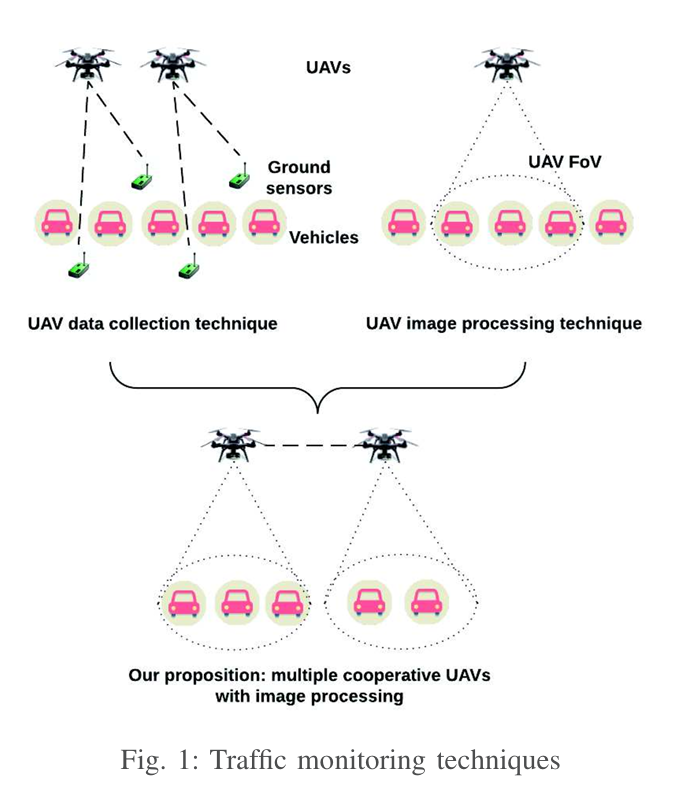
\includegraphics[width=0.7\textwidth]{Figures/Chapter3/Method4/3.png}
    \caption{Traffic monitoring techniques (Source: \cite{elloumi2018monitoring})}
    \label{fig:vehicular_mobility}
\end{figure}

\vspace{\baselineskip} % Add a line space between paragraphs

\subsection{Simulation and Results}
The study evaluates UAV-based road traffic monitoring (RTM) through simulations. Real-world taxi mobility datasets from Rome and San Francisco were initially considered but deemed unsuitable due to sparse vehicle distribution. Instead, the Opportunistic Network Environment (ONE) simulator was used to generate vehicle movement patterns based on real maps, applying Dijkstra’s shortest path algorithm. The research tested different UAV clustering methods based on distance, velocity, and direction to optimize monitoring. Simulations examined UAV coverage efficiency, event detection (speeding, congestion), and tracking methods.

\subsubsection{Key Findings}
\begin{itemize}
    \item \textbf{Fixed POI Method with Random UAV Movement}: The detection rate of speeding vehicles increases from 32\% (5 POIs) to 80.87\% (50 POIs). However, as the number of POIs increases, the time UAVs spend over a given area decreases, leading to shorter detected event durations.
    \item \textbf{Mobile Trajectory Methods}: These methods perform better, achieving up to 28.62\% coverage (Mobile POI with 50 UAVs) and a 30.09\% speeding violation detection rate (Vehicular Mobility-Based Method with 50 UAVs). Since UAVs follow mobile trajectories rather than fixed points, they can track events more accurately over time.
    \item \textbf{Impact of UAV Numbers}: For a small number of UAVs, all methods perform similarly. However, from 25 UAVs onward, the proposed methods show significant improvement. The initial estimate was that 25 UAVs would cover 10\% of targets, but with the proposed methods, the coverage rate reaches 17\%.
\end{itemize}

This table compares three UAV trajectory methods: the \textbf{Fixed Trajectory Approach}, the \textbf{Mobile POI Method}, and the \textbf{Vehicular Mobility-Based Method}. It highlights key differences in target tracking, adaptation, application domains, and UAV speed, showcasing how each approach is suited for specific monitoring tasks such as traffic surveillance, crowd tracking, or animal monitoring.

\begin{table}[H]
    \centering
    \begin{tabular}{|p{3cm}|p{4cm}|p{4cm}|p{4cm}|}
        \toprule
        \textbf{Criterion} & \textbf{Fixed Trajectory} & \textbf{Mobile POI} & \textbf{Vehicular Mobility} \\
        & \textbf{Approach} & \textbf{Method} & \textbf{Based Method} \\
        \midrule
        \textbf{Target Tracking} & Fixed Points of Interest (POIs) & Center of gravity of target groups & Pre-calculated trajectories on roads \\
        \midrule
        \textbf{Adaptation} & Static, predefined paths & Dynamic, based on target movements & Static, follows pre-generated points \\
        \midrule
        \textbf{Application Domain} & High-traffic zones (e.g., intersections) & Crowd monitoring, animal tracking, etc. & Traffic monitoring \\
        \midrule
        \textbf{UAV Speed} & Fixed & Variable, depending on group movements & Adjusted to match vehicle speeds \\
        \bottomrule
    \end{tabular}
    \caption{Comparison of Fixed Trajectory, Mobile POI, and Vehicular Mobility Based Methods}
    \label{tab:comparison_uav}
\end{table}

\vspace{\baselineskip} % Add a line space between paragraphs

\subsection{Limitations of the Method}
Despite its innovative approach, the proposed cooperative traffic monitoring system using multiple UAVs has several limitations:

\begin{itemize}
    \item \textbf{Real-Time Reporting}: The system lacks real-time capabilities for identifying and reporting speed violations to the mobile police base station. This limits its effectiveness in enforcing traffic regulations promptly.
    \item \textbf{Energy Constraints}: UAVs have limited battery life, which restricts their operational duration and requires frequent recharging or battery swaps, especially in large or remote areas.
    \item \textbf{Communication Challenges}: Maintaining stable communication links between UAVs and the ground station can be difficult, particularly in urban environments with obstacles that block or degrade signals.
    \item \textbf{Scalability Issues}: While the system performs well with a moderate number of UAVs, scaling it up to cover larger areas or more targets may require significant computational and logistical resources.
    \item \textbf{Environmental Factors}: Adverse weather conditions, such as strong winds or heavy rain, can affect UAV stability and the quality of video footage, reducing the system's reliability.
\end{itemize}

\vspace{\baselineskip} % Add a line space between paragraphs

\subsection{Conclusion}
The proposed cooperative traffic monitoring system using multiple UAVs demonstrates significant potential for urban traffic management. While challenges such as real-time speed violation reporting, energy constraints, and scalability persist, the integration of dynamic trajectory planning and clustering techniques enhances the system's effectiveness. Future work could focus on improving real-time capabilities, extending UAV battery life, and addressing communication challenges to enable large-scale implementation.

    

%%%%%%%%%%%%%%%%%%%%%%%%%%%%% Method 5 %%%%%%%%%%%%%%%%%%%%%%%%%%%%%


\section{Method 5: UAV-Assisted Emergency Vehicle Routing}
\label{sec:method5}

In a distinct approach, \cite{oubbati2019leveraging} proposed a UAV-based system specifically designed to assist emergency vehicles, such as ambulances, in identifying the optimal route through traffic to reach incident sites. The system is structured into four primary components:
\begin{itemize}
    \item \textbf{Weighting of Road Segments}: Based on traffic fluidity.
    \item \textbf{Network Organization}: Establishing a robust and energy-efficient backbone among UAVs.
    \item \textbf{Reactive Routing}: Deploying communication between the Area of Interest (AoI) and relevant services.
    \item \textbf{Path Calculation}: Determining the near-optimal path in terms of travel time to the AoI.
\end{itemize}

\vspace{\baselineskip} % Add a line space between paragraphs

\subsection{System Overview}
The proposed system enables UAVs to analyze nearby road segments and track changes in traffic conditions. UAVs communicate and collaborate by:
\begin{itemize}
    \item Exchanging messages to organize their network.
    \item Overseeing road activity to detect incidents.
    \item Promptly notifying appropriate services to support intervention.
\end{itemize}

\vspace{\baselineskip} % Add a line space between paragraphs

\subsection{System Composition}
The system is composed of \( n \) UAVs distributed across a three-dimensional (3D) space, moving randomly above various road segments. Key features of the UAVs include:
\begin{itemize}
    \item \textbf{Initial State}: Each UAV starts with a fully charged battery.
    \item \textbf{Movement Parameters}: UAVs have access to their position, speed, direction, and information about nearby UAVs.
\end{itemize}

\vspace{\baselineskip} % Add a line space between paragraphs

\subsection{UAV States and Communication}
UAVs operate in one of two states:
\begin{itemize}
    \item \textbf{Normal UAV}: Performs standard monitoring tasks.
    \item \textbf{Backbone UAV}: Acts as a communication relay for the network.
\end{itemize}

Communication between UAVs and ground vehicles is facilitated using the \textbf{IEEE 802.11p} wireless standard. To address energy constraints, the authors define three distinct levels of remaining battery capacity:
\begin{itemize}
    \item \textbf{High}: 66–100\% remaining energy.
    \item \textbf{Medium}: 33–66\% remaining energy.
    \item \textbf{Low}: 0–33\% remaining energy.
\end{itemize}

\vspace{\baselineskip} % Add a line space between paragraphs

\subsection{Operational Constraints}
Each UAV has the following operational constraints:
\begin{itemize}
    \item \textbf{Line-of-Sight (LoS) Range}: Up to 300 meters.
    \item \textbf{Altitude}: Operates at low altitudes, remaining below 300 meters.
    \item \textbf{Incident Detection}: Under clear weather conditions, UAVs can detect road incidents using image processing techniques. However, the specifics of image analysis fall outside the scope of this work.
\end{itemize}

\vspace{\baselineskip} % Add a line space between paragraphs

\subsection{Weight Calculation}
To determine the weight of a road segment, the hovering UAV collects Hello packets that are periodically exchanged between vehicles. Each intercepted Hello packet contains movement information, including the vehicle's position and speed. Regardless of its energy level or state, the UAV maintains a monitoring table to track traffic density, updating it as it receives Hello packets from vehicles traveling on a given road segment.

As illustrated in Table~\ref{tab:monitoring_table}, four UAVs (\( u_1, u_2, u_3, u_4 \)) monitor Hello packet exchanges from vehicles on four distinct road segments, each divided into three fixed zones. For instance, the monitoring table of UAV \( u_3 \) (Table~\ref{tab:monitoring_table}) is used to compute key parameters required to determine the weight of the road segment between intersections \( I_X \) and \( I_Z \).

\begin{table}[H]
    \centering
    \caption{Monitoring table of UAV \( u_3 \) (adapted from \cite{oubbati2019leveraging})}
    \label{tab:monitoring_table}
    \begin{tabular}{|c|c|c|}
        \hline
        \textbf{Zone} & \textbf{Vehicle (Position (x,y))} & \textbf{Speed (m/s)} \\
        \hline
        Zone 1 & \( v_1 \) (100.00, 5.00) & 10 \\
        \hline
        Zone 2 & \( v_2 \) (90.00, 305.00) & 8 \\
               & \( v_3 \) (90.00, 405.00) & 8 \\
        \hline
        Zone 3 & \( v_4 \) (90.00, 505.00) & 8 \\
               & \( v_5 \) (100.00, 610.00) & 14 \\
        \hline
    \end{tabular}
\end{table}

The total number of vehicles on segment \( S_{I_X I_Z} \) is given by:
\begin{equation}
    T_{S_{I_X I_Z}} = 5, \quad SP_{av} = 96 \text{ m/s}
\end{equation}

The traffic density regulation is assessed by computing the standard deviation, which reflects how vehicles are distributed across a given road segment:
\begin{equation}
    \sigma_{S_{I_i I_j}} = \sqrt{\frac{1}{S_{I_i I_j}} \sum_{i=1}^{S_{I_i I_j}} T_{Zone_i}^2 }
\end{equation}
where:
\begin{itemize}
    \item \( T_{S_{I_i I_j}} \) is the total number of vehicles in the road segment \( S_{I_i I_j} \) between intersections \( I_i \) and \( I_j \).
    \item \( \overline{T_{Zone}} \) is the average number of vehicles per zone.
    \item \( T_{Zone_i} \) is the number of vehicles in zone \( Zone_i \).
    \item \( S_{I_i I_j} \) is the number of fixed zones in the road segment \( S_{I_i I_j} \).
\end{itemize}

If \( \sigma = 0 \), vehicles are evenly distributed, implying free traffic flow. Otherwise, if \( \sigma > 0 \), vehicles tend to cluster, often due to traffic lights or congestion.

The weight of a segment \( S_{I_i I_j} \) is calculated as:
\begin{equation}
    \text{Weight} = \frac{T_{S_{I_i I_j}} +1}{d_{I_i I_j}} \times \frac{1}{SP_{av} +1}
\end{equation}
where \( d_{I_i I_j} \) is the segment length. The weight is directly proportional to \( T_{S_{I_i I_j}} \) and \( d_{I_i I_j} \). The computed weight is always non-negative and provides an indicator of traffic conditions: lower weight values correspond to better road segments.

Table~\ref{tab:weight_calculation} presents the computed weight values for different segments.

\begin{table}[H]
    \centering
    \caption{Weight Calculation Scenario (adapted from \cite{oubbati2019leveraging})}
    \label{tab:weight_calculation}
    \begin{tabular}{|c|c|c|c|c|}
        \hline
        \textbf{Segment} & \( d_{I_i I_j} \) (m) & \( T_{S_{I_i I_j}} \) & \( SP_{av} \) (m/s) & \textbf{Weight} \\
        \hline
        \( S_{I_X I_Z} \) & 1500 & 5 & 10 & 463.82 \\
        \( S_{I_Z I_Y} \) & 1500 & 0 & 0 & 0.00 \\
        \( S_{I_Y I_W} \) & 1500 & 2 & 14 & 136.05 \\
        \( S_{I_W I_X} \) & 1500 & 12 & 0 & 7468.87 \\
        \hline
    \end{tabular}
\end{table}

The segment \( S_{I_Z I_Y} \) has the lowest weight and is thus the most suitable for emergency vehicle traversal.

\vspace{\baselineskip} % Add a line space between paragraphs

\subsection{Organization and Data Routing}
To address the complexity of making a stable and reliable data transmission for alert messages, a stable backbone network is established by considering both UAV connectivity and their remaining energy levels. Graph-based modeling simplifies backbone construction by leveraging established graph theory algorithms. In this approach, UAVs and target services are represented as an undirected graph \( G(V,E) \), where \( V \) denotes vertices (UAVs and services), and \( E \) represents bidirectional links between them at a given time \( t \).

\vspace{\baselineskip} % Add a line space between paragraphs

\begin{figure}[H]
    \centering
    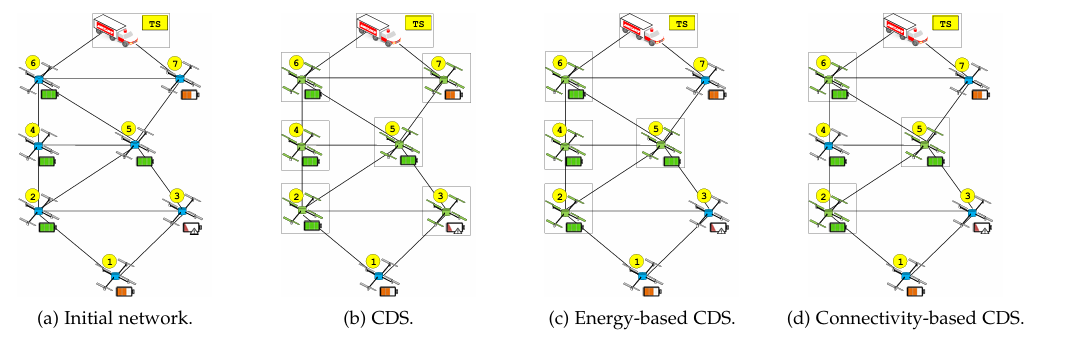
\includegraphics[width=0.7\textwidth]{Figures/Chapter3/Method5/1.png}
    \caption{Connected dominating set (CDS) formation (Source: \cite{oubbati2019leveraging})}
    \label{fig:CDS}
\end{figure}




\subsection{Connected Dominating Set (CDS) Formation}
A Connected Dominating Set (CDS) is a subset \( D \) of vertices where each non-member is connected to at least one node in \( D \), and all members of \( D \) are interconnected. Figure~\ref{fig:CDS} illustrates this process. UAVs periodically exchange Hello packets (Fig.~\ref{fig:Hello_packet_format}), which contain their ID, remaining energy (RE), mobility data (position, speed, velocity), and neighboring nodes. These details help calculate link connectivity lifetime and define network segments. A flag in the packet indicates whether a UAV belongs to the backbone (1) or not (0).

To construct the CDS, a marking process is applied:
\begin{itemize}
    \item All UAVs are initially unmarked, except the Target Service (TS), which is permanently marked.
    \item Each UAV shares its neighbor list.
    \item UAVs with two unconnected neighbors are marked.
\end{itemize}

This results in a subgraph \( M \), where \( M = G[D] \), ensuring two key properties:
\begin{itemize}
    \item \textbf{Property 1}: \( D \) forms a dominating set in \( G \).
    \item \textbf{Property 2}: \( M \) remains a connected subgraph.
\end{itemize}

Since minimizing a CDS is NP-complete, we refine \( D \) using two rules:
\begin{itemize}
    \item \textbf{Rule 1}: If a UAV \( u_i \) has a subset of its neighbors covered by another UAV \( u_j \) and \( RE_{u_i} < RE_{u_j} \), then \( u_i \) is removed from \( M \).
    \item \textbf{Rule 2}: If \( u_i \) has a lower average connectivity lifetime (ACL) than \( u_j \), it is removed. ACL is calculated using the estimated connectivity duration between UAVs.
\end{itemize}

Applying these rules optimizes the CDS, ensuring long-term connectivity while maintaining a stable backbone. The CDS updates continuously through Hello packet exchanges, providing robust network reliability.

\begin{figure}[H]
    \centering
    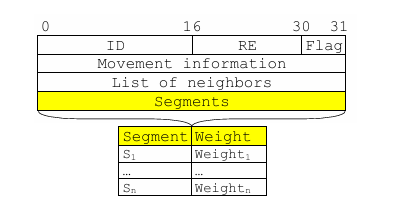
\includegraphics[width=0.7\textwidth]{Figures/Chapter3/Method5/2.png}
    \caption{Hello packet format (Source: \cite{oubbati2019leveraging})}
    \label{fig:Hello_packet_format}
\end{figure}

\vspace{\baselineskip} % Add a line space between paragraphs

\subsection{Routing}
Once the CDS is defined, an innovative routing strategy is implemented to ensure communication between the UAVs and the relevant services. This reactive approach considers two essential aspects:
\begin{itemize}
    \item Excluding UAVs with low energy levels to preserve their autonomy.
    \item Selecting routes based on link stability.
\end{itemize}

\subsubsection{Packet Format}
The RREQ (Route Request) packet contains several fields:
\begin{itemize}
    \item Transmission ID: identifier of the discovery process.
    \item NS: number of segments traversed.
    \item DelayP: transmission delay to the target service (TS).
    \item Source / TS: identifiers of the communicating nodes.
    \item Movement information: used to estimate the connection duration between UAVs.
    \item CLP (connectivity lifetime path): minimum connection duration between the UAVs in the path.
    \item REP (residual energy path): minimum energy level of the UAVs in the path.
    \item Distance: total number of UAVs traversed.
\end{itemize}

The RREP (Route Reply) packet includes these fields to inform the source about the status of the selected path. Once the RREP is received, alert transmission can begin.

\subsubsection{Routing Process}
Consider the example of an accident detected on a road. The nearest UAV immediately sends an alert to a backbone UAV, \( u_1 \). This alert contains a unique identifier, location (AoI), and the nature of the incident. Initially, only the road segments detected by the source UAV are recorded.

The UAV \( u_1 \) then broadcasts an RREQ packet to find a path to TS (hospital). At each step, information about link stability and residual UAV energy is collected. To avoid redundancies, an RREQ that has already been received with the same Transmission ID is ignored.

As soon as the first RREQ reaches TS, a short delay allows the accumulation of all available responses before selecting the optimal route. The path is chosen based on a multi-criteria score considering available energy (REP), connection duration (CLP), and number of segments traversed (NS), according to the following equation:

\[
Score = \frac{REP \times NS}{Distance} \times \frac{CLP}{DelayP}
\]

A high score indicates a reliable and stable route. Path1 (\( u_1 \rightarrow u_2 \rightarrow u_4 \rightarrow u_5 \rightarrow TS \)) is selected as it offers the best performance.


\begin{figure}[H]
    \centering
    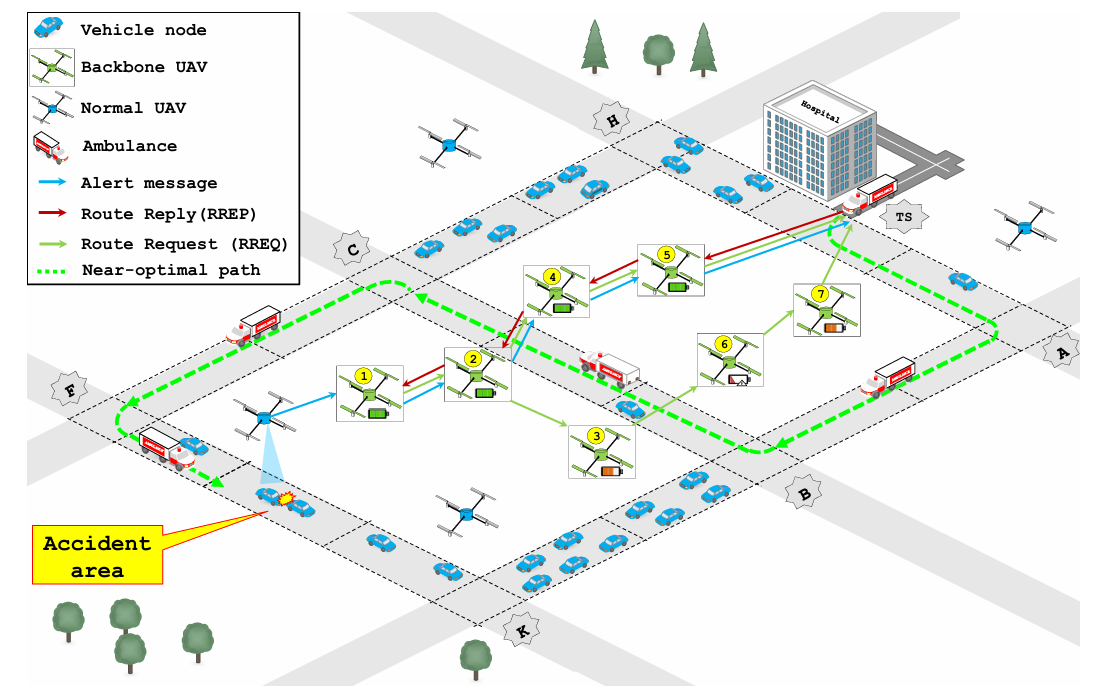
\includegraphics[width=0.7\textwidth]{Figures/Chapter3/Method5/4.png}
    \caption{alert model functioning (Source: \cite{oubbati2019leveraging})}
    \label{fig:Hello_packet_format}
\end{figure}

\subsubsection{Optimal Path Calculation to the Incident}
Once the alert is transmitted to TS, it has precise information about the incident and surrounding traffic density. Based on the weights assigned to road segments, TS calculates the best ground route to reach the AoI, ensuring a rapid emergency response.

\vspace{\baselineskip} % Add a line space between paragraphs

\subsection{Performance Evaluation}
The performance of the proposed application is evaluated through a series of experiments using NS-2, SUMO, and MobiSim for mobility generation. A test urban area of \(3 \times 3 \, \text{km}^2\) is imported from OpenStreetMap, with relevant road segments and intersections marked for simulation. Key simulation parameters are summarized in Table~\ref{tab:sim_params}.

\begin{table}[H]
    \centering
    \caption{Simulation Parameters}
    \label{tab:sim_params}
    \begin{tabular}{|l|l|}
        \hline
        \textbf{Parameter} & \textbf{Value} \\
        \hline
        Frequency Band & 5.9 GHz \\
        Transmit Power & 21.5 dBm \\
        Sensitivity & -81.5 dBm \\
        MAC Layer & IEEE 802.11p \\
        Data Rate & 1 Mbit/s \\
        Area Size & \(3 \times 3 \, \text{km}^2\) \\
        Simulation Time & 300 s \\
        Number of UAVs & [10, 100] \\
        Number of Vehicles & 100 \\
        UAV Altitude & 300 m \\
        Communication Range & 300 m \\
        Hello Interval & 0.1 s \\
        Initial Energy of UAVs & 2000 J \\
        \hline
    \end{tabular}
\end{table}

\subsubsection{Routing Performance}
Three metrics are evaluated: Packet Delivery Ratio (PDR), End-to-End Delay (EED), and Overhead (OH). The proposed routing protocol is compared with LAROD and MPGR. Results show that:
\begin{itemize}
    \item \textbf{PDR}: The proposed protocol outperforms others, increasing PDR by more than 20\% due to efficient backbone utilization.
    \item \textbf{EED}: The average delay is minimized as UAV density increases, thanks to energy-rich and well-connected routing paths.
    \item \textbf{OH}: Control overhead decreases with higher UAV density, as fewer route discoveries are needed.
\end{itemize}

\subsubsection{Energy Consumption Performance}
The remaining energy levels of 50 UAVs are analyzed. The proposed protocol demonstrates well-regulated energy consumption, as it relies on backbone UAVs with high energy levels. In contrast, LAROD and MPGR show unbalanced energy consumption, with some UAVs consuming up to 60\% more energy.

\subsubsection{Application Performance}
Experiments focus on road segment coverage, backbone UAVs, and ambulance travel time:
\begin{itemize}
    \item \textbf{Coverage}: Full road segment coverage is achieved with approximately 70 UAVs.
    \item \textbf{Backbone UAVs}: The number of backbone UAVs increases uniformly with UAV density.
    \item \textbf{Travel Time}: The proposed application provides less crowded paths, significantly reducing ambulance travel time compared to the shortest path.
\end{itemize}

\vspace{\baselineskip} % Add a line space between paragraphs

\subsection{Limitations of the Method}
Despite its innovative approach and promising results, the proposed method has several limitations that need to be addressed for practical deployment:
\begin{itemize}
    \item \textbf{Energy Constraints}: UAVs have limited battery life, which restricts their operational duration. Frequent recharging or battery replacement is required, especially in large-scale deployments.
    \item \textbf{Communication Reliability}: The system relies on IEEE 802.11p for communication, which is susceptible to interference and signal degradation in urban environments with obstacles like buildings and trees.
    \item \textbf{Line-of-Sight Dependency}: UAVs require a clear line of sight for effective communication and monitoring. This limits their effectiveness in densely built urban areas or during adverse weather conditions.
    \item \textbf{Scalability Issues}: While the system performs well with up to 100 UAVs, scaling to larger areas or higher UAV densities may introduce challenges in network organization and backbone maintenance.
    \item \textbf{Real-Time Processing}: The system assumes real-time processing of traffic data and incident detection. However, delays in data transmission or processing could impact the timeliness of emergency responses.
    \item \textbf{Regulatory Restrictions}: UAV operations are subject to strict regulations, including altitude limits, no-fly zones, and licensing requirements. These constraints could hinder widespread adoption.
    \item \textbf{Environmental Sensitivity}: The system's performance may degrade in extreme weather conditions, such as heavy rain, fog, or strong winds, which can affect UAV stability and communication.
\end{itemize}

\vspace{\baselineskip} % Add a line space between paragraphs

\subsection{Conclusion}
The proposed UAV-assisted emergency vehicle routing system demonstrates significant potential for improving emergency response times in urban environments. By leveraging UAVs for real-time traffic monitoring and dynamic route optimization, the system provides a robust solution for navigating congested road networks. However, addressing the limitations related to energy, communication, scalability, and regulatory compliance will be critical for its successful deployment and adoption.


%%%%%%%%%%%%%%%%%%%%%%%%%%%%% Method 6 %%%%%%%%%%%%%%%%%%%%%%%%%%%%%
   
    
\section{Method 6: Collaborative Hotspot Selection (CHS) for UAV-Based Traffic Surveillance}
\label{sec:method6}

In \cite{bashir2022closed}, the authors proposed a Collaborative Hotspot Selection (CHS) framework, which leverages a closed-loop control system to dynamically adjust UAV operations based on feedback from a Wireless Sensor Network (WSN). Unlike traditional open-loop systems, where UAVs follow fixed paths or remain stationary, the CHS system adapts to real-time traffic conditions, optimizing the detection of overspeeding incidents. This section provides an overview of the CHS architecture, its probabilistic model for UAV trajectory control, and its performance evaluation through simulations.

\vspace{\baselineskip} % Add a line space between paragraphs

\subsection{System Overview}
The CHS framework integrates UAVs and a WSN to monitor traffic violations, particularly overspeeding, in real-time. The system operates as follows:
\begin{itemize}
    \item \textbf{Wireless Sensor Network (WSN):} The WSN consists of Reporting Nodes (RNs) equipped with speed sensors and Helping Nodes (HNs) that facilitate communication. RNs detect overspeeding vehicles by analyzing disturbances in the Earth's magnetic field, while HNs ensure seamless data transmission between RNs, UAVs, and the Mobile Base Station (MBS).
    \item \textbf{UAV Trajectory Control:} The UAV dynamically adjusts its position based on overspeeding data collected by RNs. A probabilistic model determines the optimal hotspot for the UAV to monitor, ensuring maximum detection efficiency.
    \item \textbf{Closed-Loop Feedback:} The system continuously compares actual overspeeding incidents detected by the UAV with expected incidents reported by the WSN, enabling real-time adjustments to UAV operations.
\end{itemize}

Figure~\ref{fig:chs_architecture} illustrates the overall architecture of the CHS system.

\begin{figure}[h]
    \centering
    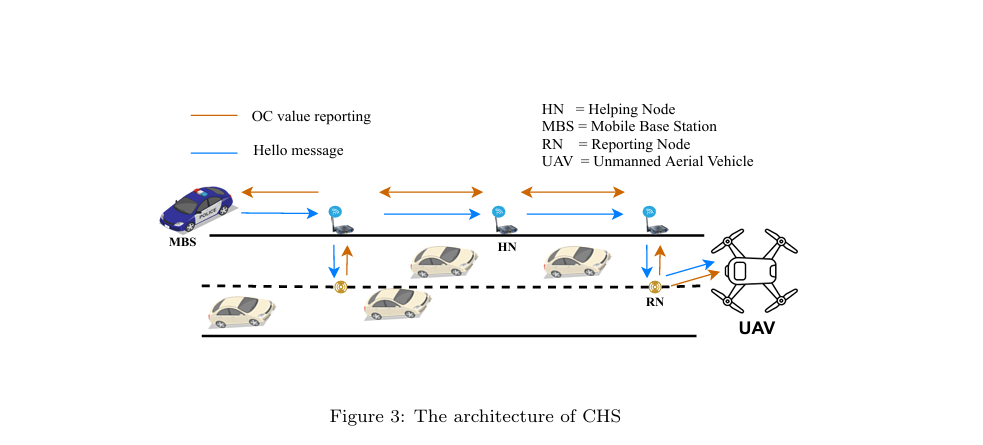
\includegraphics[width=0.7\textwidth]{Figures/Chapter3/Method6/1.png}
    \caption{CHS System Architecture (Source: \cite{bashir2022closed})}
    \label{fig:chs_architecture}
\end{figure}

\vspace{\baselineskip} % Add a line space between paragraphs

\subsection{Probabilistic Model for UAV Trajectory Control}
The CHS system employs a probabilistic approach to manage the UAV’s flight trajectory. Overspeeding incidents are modeled as a Poisson process, where the Overspeeding Count (OC) represents the average rate of violations over a given time period. The Poisson distribution function for a random variable \( Y \) is given by:

\begin{equation}
P(Y = y) = \frac{\lambda^y e^{-\lambda}}{y!}
\label{eq:poisson}
\end{equation}

where:
\begin{itemize}
    \item \( \lambda \) is the mean success rate (average OC value).
    \item \( e \) is Euler’s number.
    \item \( y \) is the actual number of overspeeding incidents in a defined time frame.
\end{itemize}

The UAV calculates the probability of detecting overspeeding incidents at each RN using the following steps:
\begin{enumerate}
    \item \textbf{Probability of Fewer Incidents:} The probability of an RN detecting fewer than \( OC_{max} \) overspeeding vehicles is calculated as:
    \begin{equation}
    Pr(Y < OC_{max}) = \sum_{y=0}^{OC_{max}-1} \frac{(OC_{rtn-1})^y e^{-OC_{rtn-1}}}{y!}
    \label{eq:prob_less}
    \end{equation}

    \item \textbf{Probability of More Incidents:} The probability of an RN detecting at least \( OC_{max} \) overspeeding vehicles is:
    \begin{equation}
    Pr(Y \geq OC_{max}) = 1 - Pr(Y < OC_{max})
    \label{eq:prob_more}
    \end{equation}

    \item \textbf{Travel Time Adjustment:} The UAV adjusts its trajectory based on the travel time between RNs, calculated as:
    \begin{equation}
    t_{r,x} = \frac{d_{r,x}}{v}
    \label{eq:travel_time}
    \end{equation}
    where \( d_{r,x} \) is the distance between RNs \( r \) and \( x \), and \( v \) is the UAV’s speed.
\end{enumerate}

The UAV uses these probabilities to determine its next position, prioritizing RNs with the highest likelihood of overspeeding incidents. Figure~\ref{fig:uav_movement} illustrates the UAV’s movement based on probabilistic calculations.

\begin{figure}[h]
    \centering
    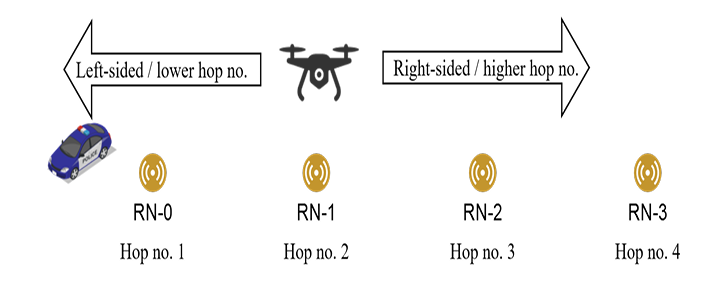
\includegraphics[width=0.7\textwidth]{Figures/Chapter3/Method6/2.png}
    \caption{Movement Control Algorithm and Hop Count Assignment (Source: \cite{bashir2022closed})}
    \label{fig:hop_numbers}
\end{figure}

\vspace{\baselineskip} % Add a line space between paragraphs

\subsection{Hop Number Allocation and Instant Reporting}
The Mobile Base Station (MBS) broadcasts hello messages to assign hop numbers to UAVs and wireless nodes. This process ensures efficient data routing and communication within the network. Key features include:
\begin{itemize}
    \item \textbf{Hop Number Assignment:} Each node updates its hop number based on the received hello message and rebroadcasts it with an incremented hop count.
    \item \textbf{Instant Reporting:} Severe speed violations are reported immediately to the MBS, while less critical violations are transmitted when the UAV is near the MBS.
\end{itemize}

Figure~\ref{fig:hop_numbers} illustrates the hop number assignment procedure.

\vspace{\baselineskip} % Add a line space between paragraphs

\subsection{Performance Evaluation}
The performance of the CHS system was evaluated through simulations using Network Simulator-2 (NS-2). Four traffic scenarios were tested to assess the system’s ability to minimize UAV movements while maximizing overspeeding detection. The results were compared with two existing methods:
\begin{itemize}
    \item \textbf{Static:} The UAV remains stationary at a fixed hotspot.
    \item \textbf{Stepwise:} The UAV follows a predefined trajectory without adapting to real-time data.
\end{itemize}

\subsubsection{Key Metrics}
The evaluation focused on three metrics:
\begin{enumerate}
    \item \textbf{Detection Rate:} The number of overspeeding incidents detected by the UAV.
    \item \textbf{Response Time:} The delay in reporting critical violations to the MBS.
    \item \textbf{Energy Efficiency:} The UAV’s energy consumption during surveillance.
\end{enumerate}

\subsubsection{Simulation Results}
\begin{itemize}
    \item \textbf{Simulation-I:} When RN-2.0 was the dominant hotspot, the Static-2.0 scheme detected the most violations. However, the CHS system performed similarly by dynamically adjusting to the hotspot.
    \item \textbf{Simulation-II:} When RN-3.9 became the dominant hotspot, Static-3.9 outperformed other static schemes, while CHS adapted effectively by relocating the UAV to RN-3.9.
    \item \textbf{Simulation-III:} With RN-5.3 as the dominant hotspot, Static-5.3 detected the most violations, while CHS maintained high detection rates by balancing movement and monitoring.
    \item \textbf{Simulation-IV:} In a dynamic scenario with shifting hotspots, CHS outperformed all static and stepwise schemes by continuously adapting to real-time data.
\end{itemize}

\begin{table}[h]
    \centering
    \caption{Simulation Parameters}
    \label{tab:simulation_params}
    \begin{tabular}{|l|c|}
        \hline
        \textbf{Parameter} & \textbf{Value} \\
        \hline
        Network size & 10 m \(\times\) 10000 m \\
        UAV speed & 15 m/s \\
        Transmission range & 100 m \\
        Number of wireless nodes & 78 \\
        Number of vehicles & 200–300 \\
        Vehicle speed range & 13–27 m/s \\
        OC reporting interval & 100 s \\
        Simulation time & 0–2500 s \\
        \hline
    \end{tabular}
\end{table}

\vspace{\baselineskip} % Add a line space between paragraphs

\subsection{Limitations and Challenges}
While the CHS system demonstrates significant potential, it faces several limitations:
\begin{itemize}
    \item \textbf{Energy Constraints:} UAVs have limited battery life, which restricts their operational duration. Frequent recharging or battery replacement is required, especially in large-scale deployments.
    \item \textbf{Communication Reliability:} The system relies on IEEE 802.11p for communication, which is susceptible to interference and signal degradation in urban environments.
    \item \textbf{Environmental Sensitivity:} Adverse weather conditions, such as heavy rain or strong winds, can affect UAV stability and communication.
    \item \textbf{Real-Time Processing:} The system assumes real-time processing of traffic data, but delays in data transmission or processing could impact its responsiveness.
    \item \textbf{Regulatory Restrictions:} UAV operations are subject to strict regulations, including altitude limits and no-fly zones, which could hinder widespread adoption.
\end{itemize}

\vspace{\baselineskip} % Add a line space between paragraphs


%%%%%%%%%%%%%%%%%%%%%%%%%%%%% Conclusion %%%%%%%%%%%%%%%%%%%%%%%%%%%%%


\section{Conclusion}

The six methods discussed in this chapter illustrate the diverse and innovative approaches to UAV-based traffic monitoring, each addressing specific challenges in traffic surveillance and management. From early systems like the Airborne Traffic Surveillance System (ATSS) to advanced frameworks such as Collaborative Hotspot Selection (CHS), these methods demonstrate the potential of UAVs to revolutionize traffic monitoring by providing real-time, adaptive, and scalable solutions. Key advancements include the integration of 5G technology for high-speed communication, probabilistic models for dynamic UAV trajectory control, and cooperative systems that leverage multiple UAVs for comprehensive coverage.

\vspace{\baselineskip} % Add a line space between paragraphs

Despite their promise, these methods face several challenges that must be addressed for practical deployment. Energy constraints, communication reliability, and regulatory restrictions remain significant barriers to the widespread adoption of UAV-based traffic monitoring systems. Additionally, environmental factors such as adverse weather conditions and line-of-sight limitations can impact system performance. However, ongoing advancements in UAV technology, artificial intelligence, and wireless communication networks offer promising avenues for overcoming these challenges.

\vspace{\baselineskip} % Add a line space between paragraphs

In conclusion, UAV-based traffic monitoring systems represent a significant leap forward in traffic management, offering unparalleled flexibility, efficiency, and adaptability. By addressing the limitations of traditional systems and leveraging the unique capabilities of UAVs, these methods pave the way for smarter, safer, and more efficient urban transportation networks. As research and development in this field continue, the integration of UAVs into traffic monitoring systems is expected to play a pivotal role in shaping the future of intelligent transportation systems.
